\documentclass{beamer}
\usepackage{graphics}
\usepackage{epsfig}
\usepackage{multicol}
\usepackage{pifont}
\setbeamertemplate{navigation symbols}{}
\newcommand{\RR}{\ensuremath{\mathbb{R}}}
\newcommand{\NN}{\ensuremath{\mathbb{N}}}
\newcommand{\QQ}{\ensuremath{\mathbb{Q}}}
\newcommand{\CC}{\ensuremath{\mathbb{C}}}
\newcommand{\ZZ}{\ensuremath{\mathbb{Z}}}
\newcommand{\TT}{\ensuremath{\mathbb{T}}}
\newcommand{\HH}{\ensuremath{\mathbb{H}}}
\DeclareMathOperator{\Min}{Min}
\DeclareMathOperator{\Dom}{Dom}
\DeclareMathOperator{\vol}{vol}
\DeclareMathOperator{\Aut}{Aut}
\DeclareMathOperator{\Stab}{Stab}
\DeclareMathOperator{\Sym}{Sym}
\DeclareMathOperator{\Grp}{Grp}
\DeclareMathOperator{\HYP}{HYP}
\DeclareMathOperator{\CUT}{CUT}
\DeclareMathOperator{\GL}{GL}
\DeclareMathOperator{\AGL}{AGL}
\DeclareMathOperator{\Id}{Id}
\DeclareMathOperator{\mint}{min}
\DeclareMathOperator{\vertt}{vert}
\DeclareMathOperator{\conv}{conv}
\DeclareMathOperator{\rank}{rank}

\def\QuotS#1#2{\leavevmode\kern-.0em\raise.2ex\hbox{$#1$}\kern-.1em/\kern-.1em\lower.25ex\hbox{$#2$}}

\begin{document}
\title{Hindcasting surface currents in the Adriatic}
\author{
\begin{center}
\textcolor{red}{\large Mathieu Dutour Sikiri\'c}\\[2mm]
\textcolor{red}{Rudjer Bo\u skovi\'c Institute, Croatia}\\[2mm]
\textcolor{red}{and Universit\"at Rostock}
\end{center}
}


%\author{
%{\small
%\begin{center}
%\textcolor{red}{\large Mathieu Dutour Sikiri\'c}\\[2mm]
%\textcolor{red}{Rudjer Boskovic Institute, Croatia}
%\textcolor{red}{\large Aron Roland}\\[2mm]
%\textcolor{red}{Institut of Hydraulic Engineering, Darmstadt}\\[2mm]
%\textcolor{red}{\large Igor Toma\u zi\'c}\\[2mm]
%\textcolor{red}{Rudjer Boskovic Institute, Croatia}
%\textcolor{red}{\large Ivica Janekovi\'c}\\[2mm]
%\textcolor{red}{Rudjer Boskovic Institute, Croatia}
%\textcolor{red}{\large Milivoj Kuzmi\'c}\\[2mm]
%\textcolor{red}{Rudjer Boskovic Institute, Croatia}
%\end{center}
%}
%}
\date{\today} 
\frame{\titlepage} 








\frame{
\begin{center}
\begin{tabular*}{7cm}{c}
\\[-0.5cm]
{\Huge \textcolor{blue}{I. }\textcolor{red}{Wave modelling}}
\end{tabular*}
\end{center}
}

\frame{
  \frametitle{Linear water wave theory I: setting}
The basic assumptions of linear water wave theory are:
\begin{itemize}
\item The velocities and free surface elevation are small.
\item The depth $h$ is uniform.
\item The fluid has no viscosity, is incompressible and irrotational.
\end{itemize}
\begin{center}
\resizebox{6cm}{!}{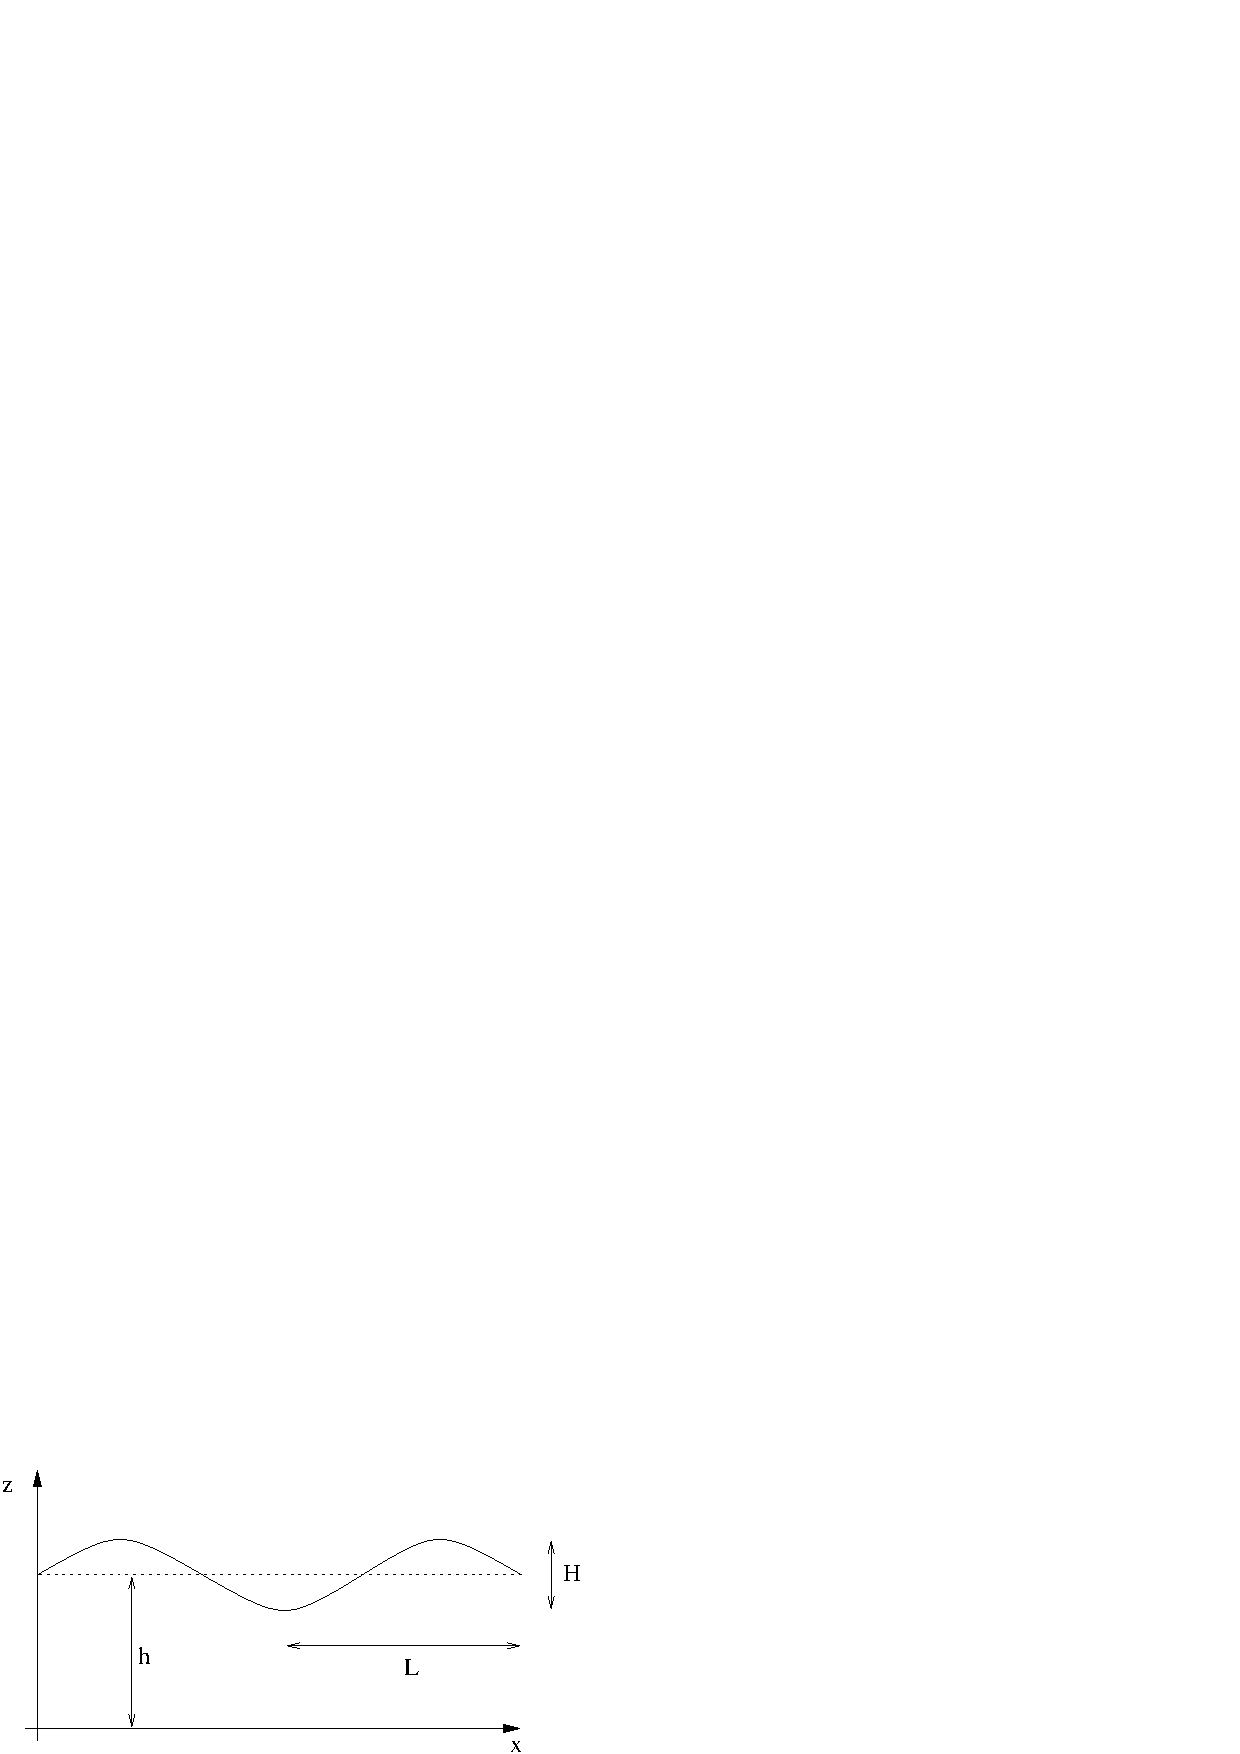
\includegraphics{FIG_wave/WaveSetting.pdf}}\par
\end{center}
We also call $T$ the wave period and define $\omega=\frac{2\pi}{T}$ and $k=\frac{2\pi}{L}$.
}


\frame{
  \frametitle{Linear water wave theory II: solution}
Under the above assumptions, it is possible to derive explicit formulas for the free surface $\xi$ and velocity $(u,w)$
\begin{equation*}
\xi=\frac{H}{2} \sin\left(2\pi \left(\frac{x}{L}-\frac{t}{T}\right)+ \phi\right)
\mbox{~and~}
(u,w)=\left(\frac{\partial \phi}{\partial x}, \frac{\partial \phi}{\partial z}\right)
\end{equation*}
with
\begin{equation*}
\phi(x,z)=\frac{g H}{2\omega} \frac{\cosh (k(z+h))}{\cosh(kh)} \sin\left(2\pi \left(\frac{x}{L}-\frac{t}{T}\right)+ \phi\right).
\end{equation*}
The wave period $T$ and wave length $L$ satisfies the dispersion relation
\begin{equation*}
\omega^2 = g k  \tanh( kh)
\end{equation*}
}






\frame{
  \frametitle{Linear water wave theory III: Stokes drift}

\begin{itemize}
\item The above expressions for velocities are given in an Eulerian fixed frame.
\item Integrated over a long time, the velocities have zero mean.
\item But if one considers a Lagrangian viewpoint, i.e. follows the particles then there is a movement:
\begin{center}
\resizebox{7cm}{!}{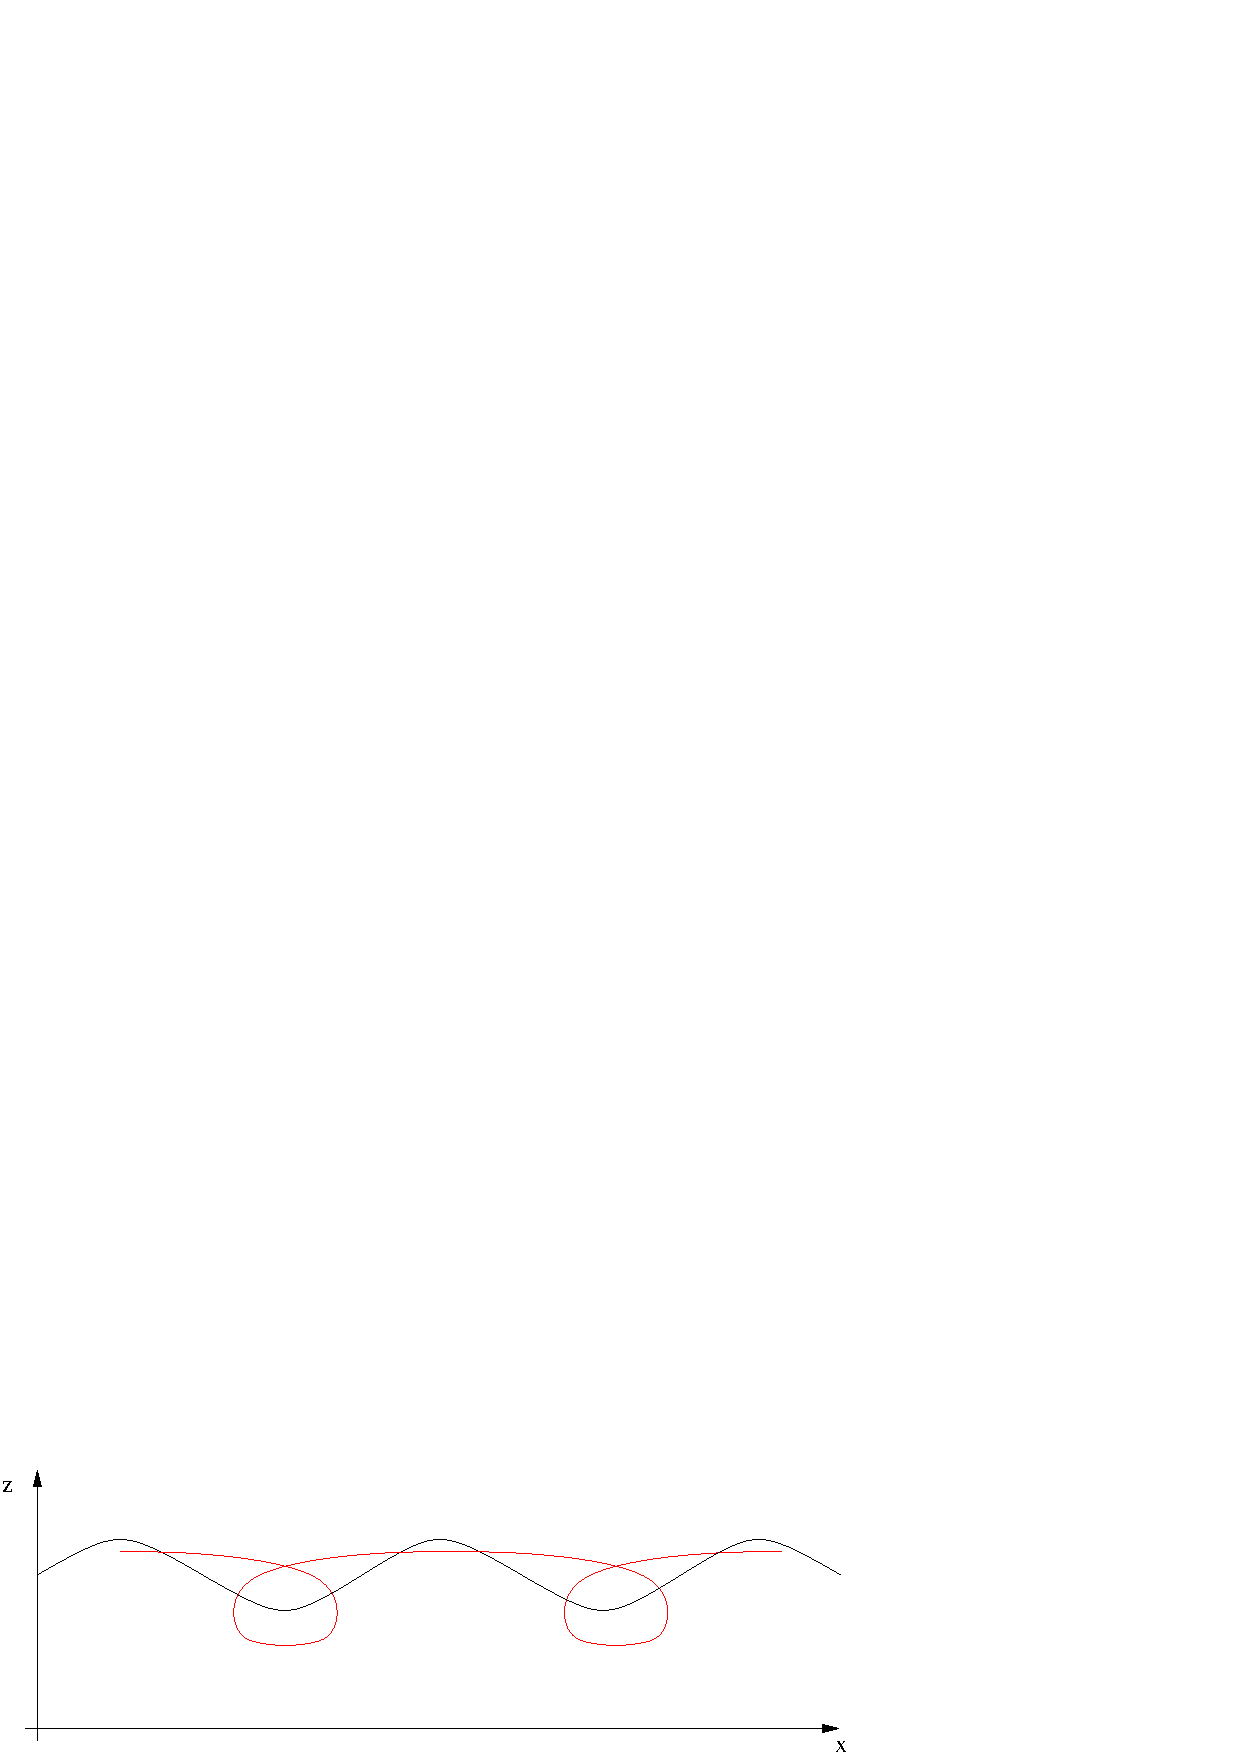
\includegraphics{FIG_wave/StokesDrift.pdf}}\par
\end{center}
\item A simplified formula for the resulting velocity is the Stokes drift
\begin{equation*}
U_{S} = \frac{1}{2} \left(\frac{\pi H}{L}\right)^2 \frac{\omega}{k} \frac{\cosh(2k(z+h))}{\sinh^2(kh)}
\end{equation*}

\end{itemize}
}





\frame{
  \frametitle{Stochastic wave modelling}

\begin{itemize}
\item Oceanic models are using grids (structured or unstructured) of size $1km\leq d\leq 10km$ to simulate the ocean
\item But oceanic waves have a typical wavelength $2m$ $\leq$ $L$ $\leq$ $100m$. So, we cannot resolve waves in the ocean.
\item But if one uses phase averaged models and uses stochastic assumptions
then it is possible to model waves by a spectral wave action density
$N({\bf x},{\bf k})$
\item This density satisfies a Wave Action Equation (\textcolor{red}{WAE}) which represents advection, refraction, frequency shifting and source terms:
\begin{equation*}
\frac{\partial N}{\partial t} + \nabla_x(({\bf c}_g+{\bf u}_A)N) + \nabla_k(\dot{k} N) 
 + \nabla_{\theta}(\dot{\theta} N) = S_{tot}
\end{equation*}
with
\begin{equation*}
S_{tot} = S_{in} + S_{nl3} + S_{nl4} + S_{bot} + S_{ds} + S_{break} + S_{bf}
\end{equation*}
\end{itemize}
}




\frame{
  \frametitle{Doppler shift}
\begin{itemize}
\item Suppose that we have a uniform current ${\bf u}$ then the dispersion relation is changed to
\begin{equation*}
\sigma^2 = g k  \tanh( kh) \mbox{~and~} \omega = \sigma + {\bf k}\cdot {\bf u}
\end{equation*}
with $\sigma$ the intrinsic frequency and $\omega$ the absolute frequency.
\item In the case of a sheared current, the Doppler shift relation changes to
\begin{equation*}
\omega = \sigma + {\bf k}\cdot\int_{z=-h}^{z=\xi} {\bf u} \frac{2k\cosh(2k(z+h))}{\sinh(2kD)} dz
\end{equation*}
\item The advection velocity ${\bf u}_A$ is usually approximated by the surface current velocity. There is unfortunately no Wave Action Equation in the case of sheared currents.
\end{itemize}
}


\frame{
  \frametitle{Wave coupling}

\begin{itemize}
\item Wave models use surface currents for the advection of wave energy and
the free surface enters into the dispersion relation.
\item On the other hand oceanic model can use wave information to:
\begin{itemize}
\item Compute the Stokes drift (current induced by waves, a nonlinear effect).
\item Compute the wave radiation pressure term in the primitive equation.
\item Improve the computation of the surface stress, turbulence.
\item Be used in sediment transport models.
\end{itemize}
\item Thus it makes sense to have oceanic and wave models coupled both ways. We chose to work with the {\tt ROMS} model (a finite difference model) and the {\tt WWM} model (a finite element model by Aron Roland).
\end{itemize}
\begin{center}
\resizebox{4cm}{!}{\includegraphics{FIG_wave/Model_Coupling.pdf}}\par
\end{center}


}







\frame{
  \frametitle{Stokes drift}
\begin{itemize}
\item For a phase averaged wave model we can define the horizontal Stokes drift as an integral over the spectrum ($E({\bf k}) = \sigma N({\bf k})$):
\begin{equation*}
(u,v)_{s} = \int_{\bf k} \frac{E({\bf k}) }{2\sinh^2(kD)}\sigma {\bf k}\cosh(2k(z+h)) d{\bf k}.
\end{equation*}
Note that the formula is actually an approximation assuming that the current shear is small. See Ardhuin (2008) for higher order formulas.
\item Now, we also need to introduce the vertical Stokes drift. This term is zero in the case of linear wave theory ($h$, $H$ and $L$ constant) but non-zero in general. The Stokes drift satisfies 
\begin{equation*}
\frac{\partial u_s}{\partial x} + \frac{\partial v_s}{\partial y} + \frac{\partial w_s}{\partial z} = 0
\end{equation*}
and so we can get $w_s$ by vertical integration from the bottom.
\end{itemize}
}




\frame{
  \frametitle{Generalized Lagrangian mean}
\begin{itemize}
\item The idea is to decompose the current as ${\bf u}_{tot} = {\bf u} + {\bf u}_{wave} + {\bf u}_{turb}$ with ${\bf u}$ the steady motion, ${\bf u}_{wave}$ the wave motion and ${\bf u}_{turb}$ the microscopic turbulent motion.
\item Under the assumption that ${\bf u}_{turb}$ is uncorrelated to other motion, we have to investigate the relation between ${\bf u}_{wave}$ and ${\bf u}$.
\item We can thus introduce a new particular derivative operator
\begin{equation*}
\frac{D}{Dt} = \frac{\partial }{\partial t} + 
(u+u_{S}) \frac{\partial }{\partial x} +
(v+v_{S}) \frac{\partial }{\partial y} +
(w+w_{S}) \frac{\partial }{\partial z}
\end{equation*}
and the equation for tracers $T$ (i.e. salinity, temperature, turbulent kinetic energy, etc.) is then
\begin{equation*}
\frac{D T}{Dt} = C(T) + D(T)
\end{equation*}
with $C(T)$ the source and sink term and $D(T)$ the diffusion term.

\end{itemize}
}





\frame{
  \frametitle{Equations of the Bennis/Ardhuin 2011 formulation I}

\begin{itemize}
\item For the conservation of momentum we have the equation
\begin{equation*}
\frac{D {\bf u}}{D t} = {\bf F}_{pres} + {\bf F}_{turb} + {\bf F}_{cor} + {\bf F}_{wave} + {\bf F}_{bottom} + {\bf F}_{surf}
\end{equation*}
where ${\bf F}_{pres}$ and ${\bf F}_{turb}$ are the pressure and turbulence terms respectively, while ${\bf F}_{cor}=f_{cor} (v + v_s, -u-u_s)$ is the Coriolis term with $f_{cor}$ the Coriolis factor.
\item The wave pressure term is a 
\begin{equation*}
{\bf F}_{wave} = u_s {\bf \nabla} u + v_s {\bf \nabla} v - {\bf \nabla} J
%\left\{\begin{array}{rcl}
%F_{wave, x} &=& \frac{\partial v}{\partial x} v_s + \frac{\partial u}{\partial x} u_s - \frac{\partial J}{\partial x},\\
%F_{wave, y} &=& \frac{\partial v}{\partial y} v_s + \frac{\partial u}{\partial y} u_s - \frac{\partial J}{\partial x}.
%\end{array}\right.
\end{equation*}
with $J$ the 2D wave pressure term given by 
\begin{equation*}
J = \int_{\bf k} g\frac{k E({\bf k})}{\sinh(2kD)} d{\bf k}. 
\end{equation*}

\end{itemize}
}






\frame{
  \frametitle{Equations of the Bennis/Ardhuin 2011 formulation II}
\begin{itemize}
\item The equation for the free surface is changed to
\begin{equation*}
\frac{d\xi}{dt} + (u + u_s) \frac{d\xi}{dx} + (v+v_s)\frac{d\xi}{dy} = w + w_s
\end{equation*}
\item Boundary conditions are changed from $u=0$ to $u=-u_s$ and similarly for other kind of boundary conditions.
\item The Stokes drift must also be added to the computation of floats trajectories.
\item (Ardhuin, 2008) actually proposed a more complex system of equations with higher order terms.
\item (Mellor, 2003) proposed some expression for the baroclinic stress but some incoherent results were obtained with it.
\item (Longuet-Higgins, 1953) derived an expression for the barotropic stress induced by waves.


%\item (Ardhuin, 2007) proposed a new set of equations with the basic prototype for the tracer equation:
%\begin{equation*}
%\frac{\partial T}{\partial t} + 
%(u+u_{S}) \frac{\partial T}{\partial x} +
%(v+v_{S}) \frac{\partial T}{\partial y} +
%(w+w_{S}) \frac{\partial T}{\partial z} = S_T
%\end{equation*}
%with $(u,v,w)_S$ being the Stokes drift and $S_T$ the source of the tracer.
%\item The boundary condition for momentum changes from $u=0$ to $u=-u_S$.
\end{itemize}
}

\frame{
  \frametitle{Surface stress}
\begin{itemize}
\item Surface stress is a key unknown in many oceanigraphic simulations.
\item Many formulas depending on the wind ${\bf u}_{10m}$ have been proposed and the Charnock parameter was introduced
\begin{equation*}
\alpha = z_0 \frac{g}{u_{*}^2}
\end{equation*}
with $z_0$ the roughness length and $u_{*}$ the friction velocity. But the variability remains very large.
\item Janssen (1989) proposed to decompose the stress into
\begin{equation*}
\tau = \tau_{viscous}  + \tau_{wave} + \tau_{high.\,freq.}
\end{equation*}
\item The term $\tau_{viscous}$ is negligible. 
\item Janssen (1989) proposed a parameterization of the high frequency stress
\item And $\tau_{wave}$ is obtained as an integral over the wind input formula of the wave model.

\end{itemize}
}




\frame{
\begin{center}
\begin{tabular*}{7cm}{c}
\\[-0.5cm]
{\Huge \textcolor{blue}{II. }\textcolor{red}{Numerical}}\\[4mm]
{\Huge \textcolor{red}{and computer}}\\[4mm]
{\Huge \textcolor{red}{aspects}}
\end{tabular*}
\end{center}
}






\frame{
  \frametitle{{\tt MPI} based models}
\begin{itemize}
\item Geophysical models are dominated by the {\tt MPI} parallel formalism. In it the program is split into several nodes that communicate by {\tt Recv}/{\tt Send} commands.
\item As a consequence, when parallelizing models, it is best to have at the beginning an assignment in {\tt MyColor} of the nature of the node, then call
\begin{center}
{\tt MPI\_COMM\_SPLIT(MPI\_COMM\_WORLD, MyColor, MyCOMM)}
\end{center}
From that point we have a new communicator {\tt MyCOMM} that can be used inside of the existing code by replacing the {\tt MPI\_COMM\_WORLD}
\item So, apart from exchanging data, merging two {\tt MPI} programs together takes only a few lines.
\end{itemize}
}


\frame{
  \frametitle{Model coupling library, {\tt PGMCL} }
\begin{itemize}
\item The exchange between models requires the sending of data between them.
\item A priori the grids are different, the model nature may be different (Structure/Unstructured grids) and so interpolation is needed between the models.
\item There are several existing libraries {\tt MCT}, {\tt OASIS}, {\tt PALM}, etc but when considering them, they appear all relatively complicated.
\item We considered {\tt MCT} and it appeared to be impossible to achieve the goals that we wanted (optimal exchanges, interpolation, performance, etc.).
\item Henceforth, we designed our own library {\tt PGMCL} (Parallel Geophysical Model Coupling Library) for coupling models.
\item After declarations, the commands become as simple as
\begin{center}
{\tt CALL MPI\_INTERP\_SEND(TheArr\_WAVtoOCN, Hwave)}\\
{\tt CALL MPI\_INTERP\_RECV(TheArr\_WAVtoOCN, Hwave)}
\end{center}

\end{itemize}
}




\frame{
  \frametitle{Coupling of {\tt WAM} and {\tt COSMO}}
\begin{itemize}
\item The {\tt WAM} model, originally the first $3^{rd}$ generation wave model, is a wave model used by many institutions  in the world.
\item The {\tt COSMO} model is based on the Lokall modell of DWD.
\item Both are finite difference models that are coupled via {\tt PGMCL}
\begin{itemize}
\item The atmospheric model provides the wind and air density to wave model.
\item The wave model provides the Charnock coefficient to the atmospheric model.
\end{itemize}
\item Results on the Mediterranean indicate a slight decrease of wind magnitude.

\end{itemize}
Work done in collaboration with P. Janssen/J. Bidlot (ECMWF), L. Cavaleri (ISMAR), L. Torrisi (CNMCA, Italian Nat. Met. Center) and A. Roland (TU Darmstadt)
}






\frame{
  \frametitle{WaveWatch III coarse/fine grids}

\begin{itemize}
\item The WaveWatch III model is another wave model used by several oceanographic institutions. It can work with nested grids, which are finite difference or finite element.
\item My contribution was the implementation of coarse $\rightarrow$ fine (interpolation) and fine $\rightarrow$ coarse (averaging, scrip library) in the case (FD/FE).
\end{itemize}
\begin{center}
\begin{minipage}{3.9cm}
\centering
\resizebox{3.9cm}{!}{\includegraphics{WavePic/MultiFD_FE_atp5/MultGrid.png}}\par
\end{minipage}
\begin{minipage}{3.3cm}
\centering
\resizebox{3.3cm}{!}{\includegraphics{WavePic/MultiFD_FE_atp5/FD_Hwave_ww0009_20071102_000000.png}}\par
\end{minipage}
\begin{minipage}{3.3cm}
\centering
\resizebox{3.3cm}{!}{\includegraphics{WavePic/MultiFD_FE_atp5/FE_Hwave_ww0009_20071102_000000.png}}\par
\end{minipage}

\end{center}
Work done with F. Ardhuin (IFREMER), E. Rogers (NRL) and A. Roland (TU Darmstadt)
}




\frame{
  \frametitle{Numerics of the coupling}
\begin{itemize}
\item The mathematical expressions occurring in wave modelling are for example
\begin{equation*}
\frac{\cosh(2k z)}{\sinh(2k h)}
\end{equation*}
\item This kind of function is very singular. Their large values are concentrated on the surface. On the other hand it satisfies a specific integral property:
\begin{equation*}
\frac{1}{h} \int_0^h \frac{\cosh(2k z)}{\sinh(2k h)} dz=\frac{1}{2kh}
\end{equation*}
which has to be reproduce in the model.
\item The solution that we choose is for every vertical cell of the model, to compute explicitly the integral and put the average value at the relevant point.
\item This also applies to the computation of the $S_{xx}$ quantities of Mellor's formulation of wave physics.
\end{itemize}
}



\frame{
  \frametitle{Computation of the Stokes drift}

\begin{center}
\begin{minipage}{5.0cm}
\centering
\resizebox{4.4cm}{!}{\includegraphics{DrifterPicture/TRC_Stokes_mod.png}}\par
\end{minipage}
\begin{minipage}{5.3cm}
\centering
\resizebox{5.0cm}{!}{\includegraphics{DrifterPicture/INT_Stokes.png}}\par
\end{minipage}
\end{center}
For $MSC$ frequencies, $MDC$ directions, $N$ vertical levels and $M$ grid level points the computation of the Stokes drift is takes  $MSC\times MDC\times N\times M$ operations.
We can reduce it to $M\times (MDC + MSC\times N)$ but that is still large.
By using significant wave height, mean wave height and direction we can reduce further the computation but then one misses the directional spreading and gets wrong results.
}






\frame{
  \frametitle{Grid subdivizion schemes}
\begin{itemize}
\item Our standard interpolation strategy is to subdivide the squares in two triangles. Then near the coast, we add some more triangles.
\begin{center}
\begin{minipage}{3.2cm}
\centering
\resizebox{2.5cm}{!}{\includegraphics{FIG_wave/Subdiv_straightforward_red.pdf}}\par
\end{minipage}
\begin{minipage}{3.2cm}
\centering
\rotatebox{90}{\resizebox{2.5cm}{!}{\includegraphics{FIG_wave/Subdiv_coast.pdf}}}\par
\end{minipage}
\end{center}
\item Those additional triangles allow us to respect the straits and isthmus of the original grid.
\begin{center}
\begin{minipage}{3.2cm}
\centering
\rotatebox{90}{\resizebox{2.5cm}{!}{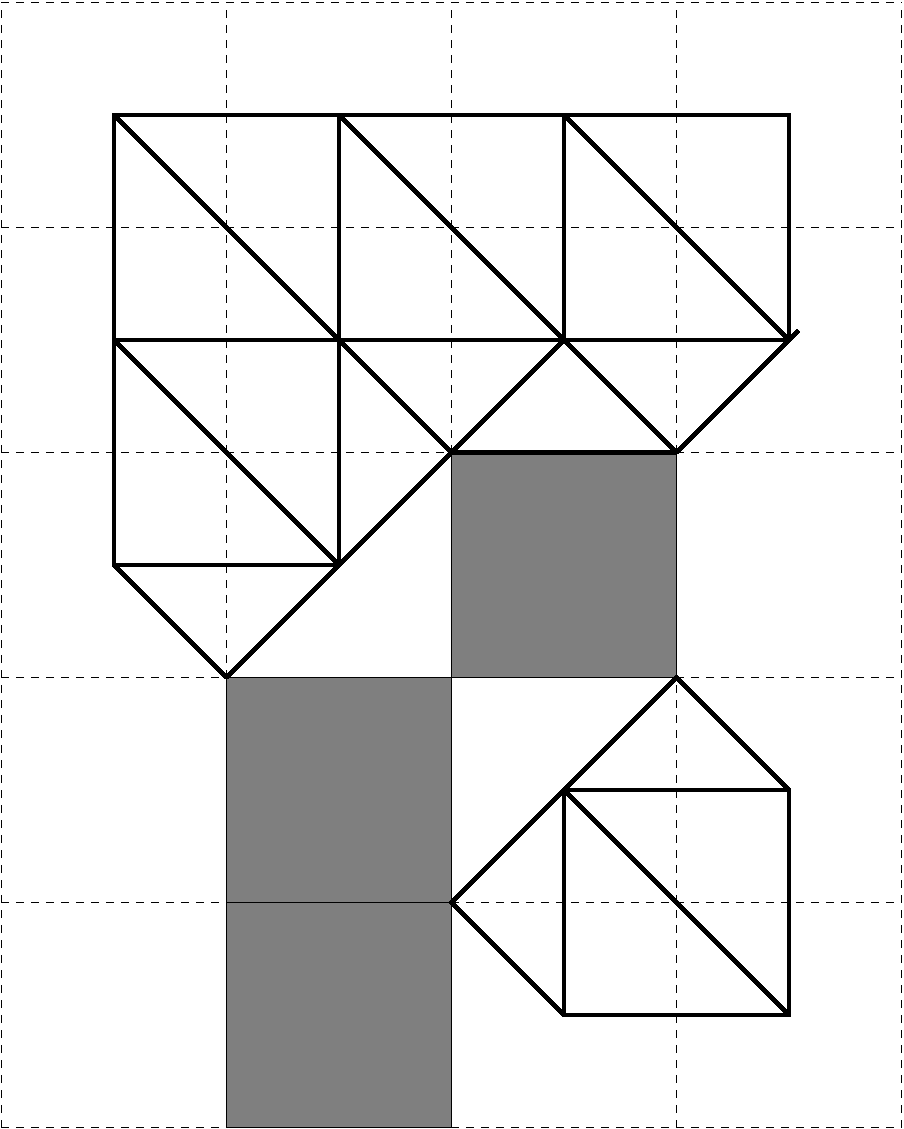
\includegraphics{FIG_wave/Subdiv_isthmus.pdf}}}\par
\end{minipage}
\begin{minipage}{3.2cm}
\centering
\rotatebox{90}{\resizebox{2.5cm}{!}{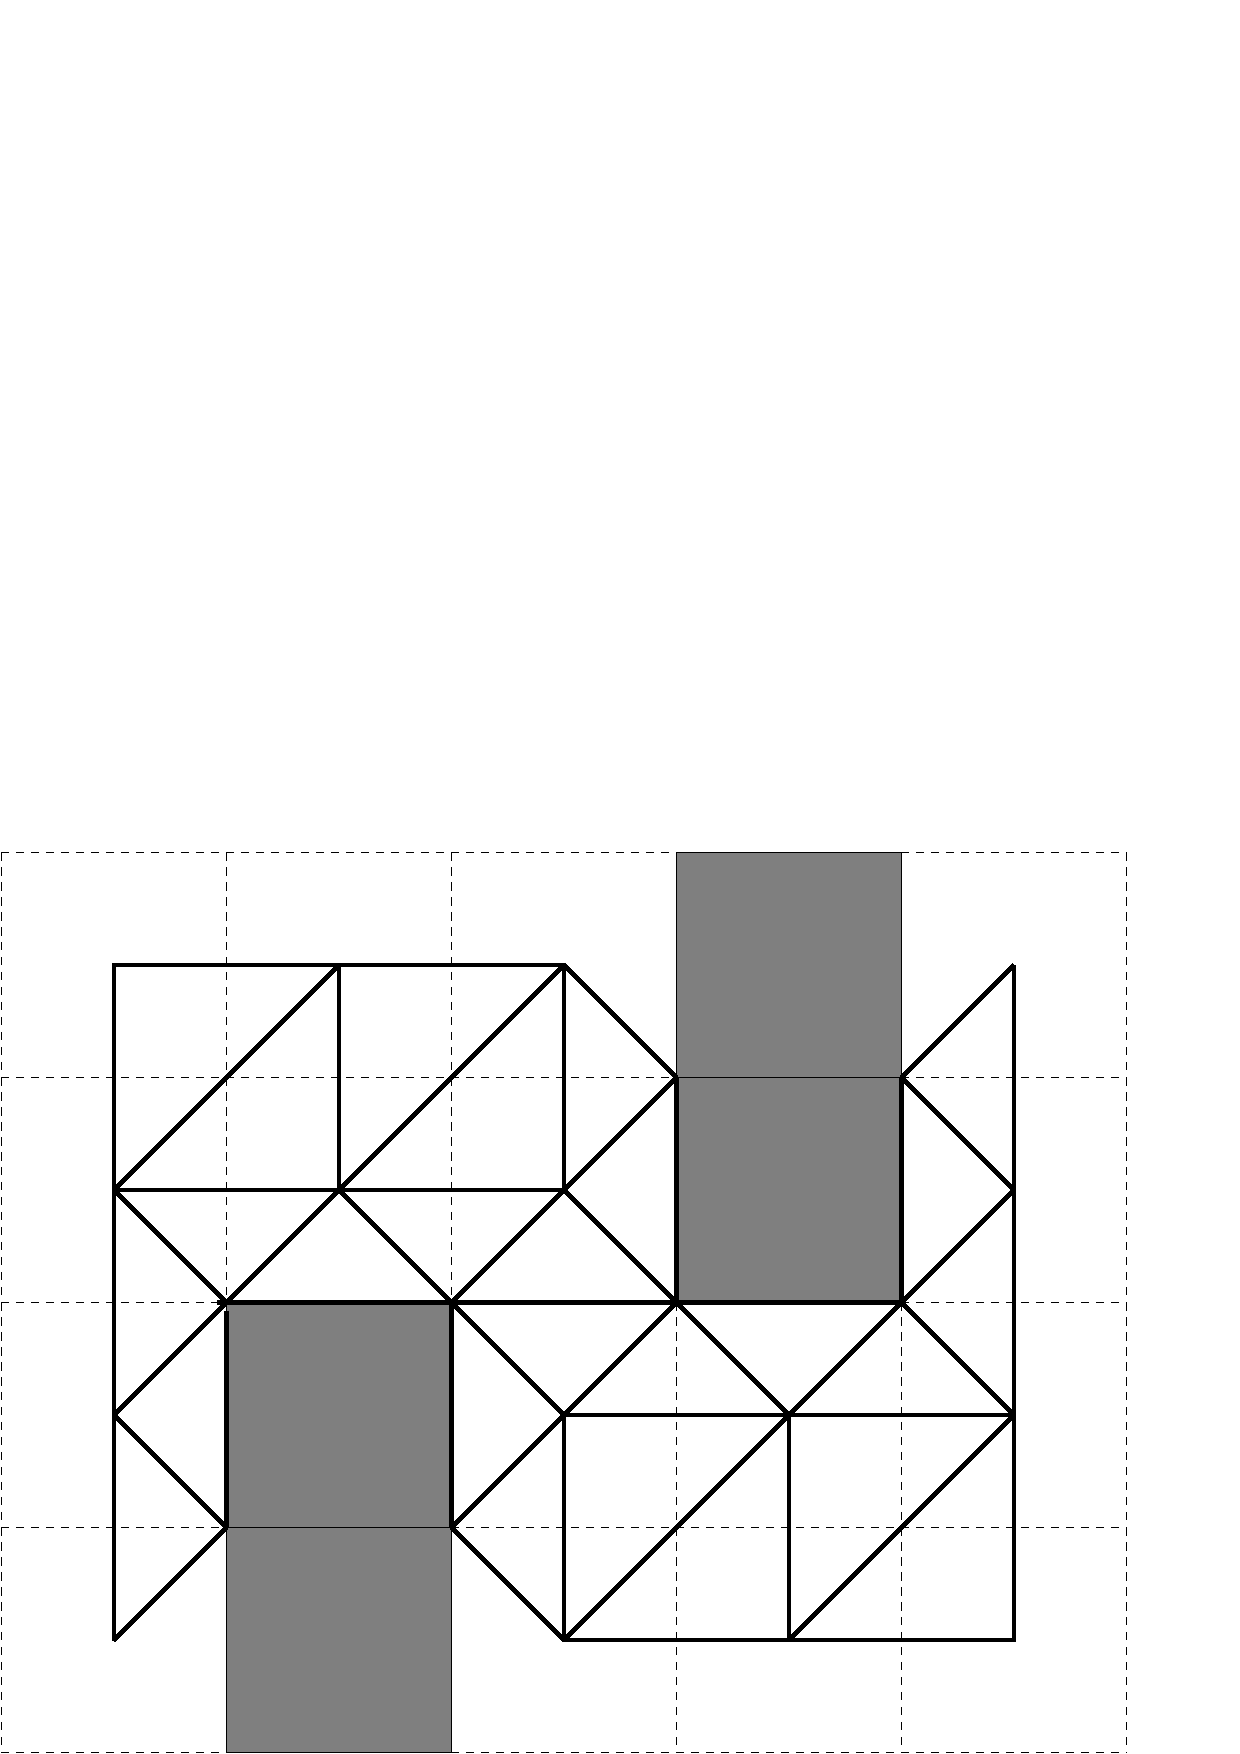
\includegraphics{FIG_wave/Subdiv_strait.pdf}}}\par
\end{minipage}
\end{center}
\item But the system also allows some finite element grid to be used.
\end{itemize}
}















\frame{
\begin{center}
\begin{tabular*}{7cm}{c}
\\[-0.5cm]
{\Huge \textcolor{blue}{III. }\textcolor{red}{Idealized test cases}}
\end{tabular*}
\end{center}
}




\frame{
  \frametitle{Shoaling idealized test case I}
\begin{itemize}
\item For the shoaling idealized test case, a wave of period $1.5s$ arrives on a beach and breaks:
\begin{center}
\begin{minipage}{9.2cm}
\centering
\resizebox{7.0cm}{!}{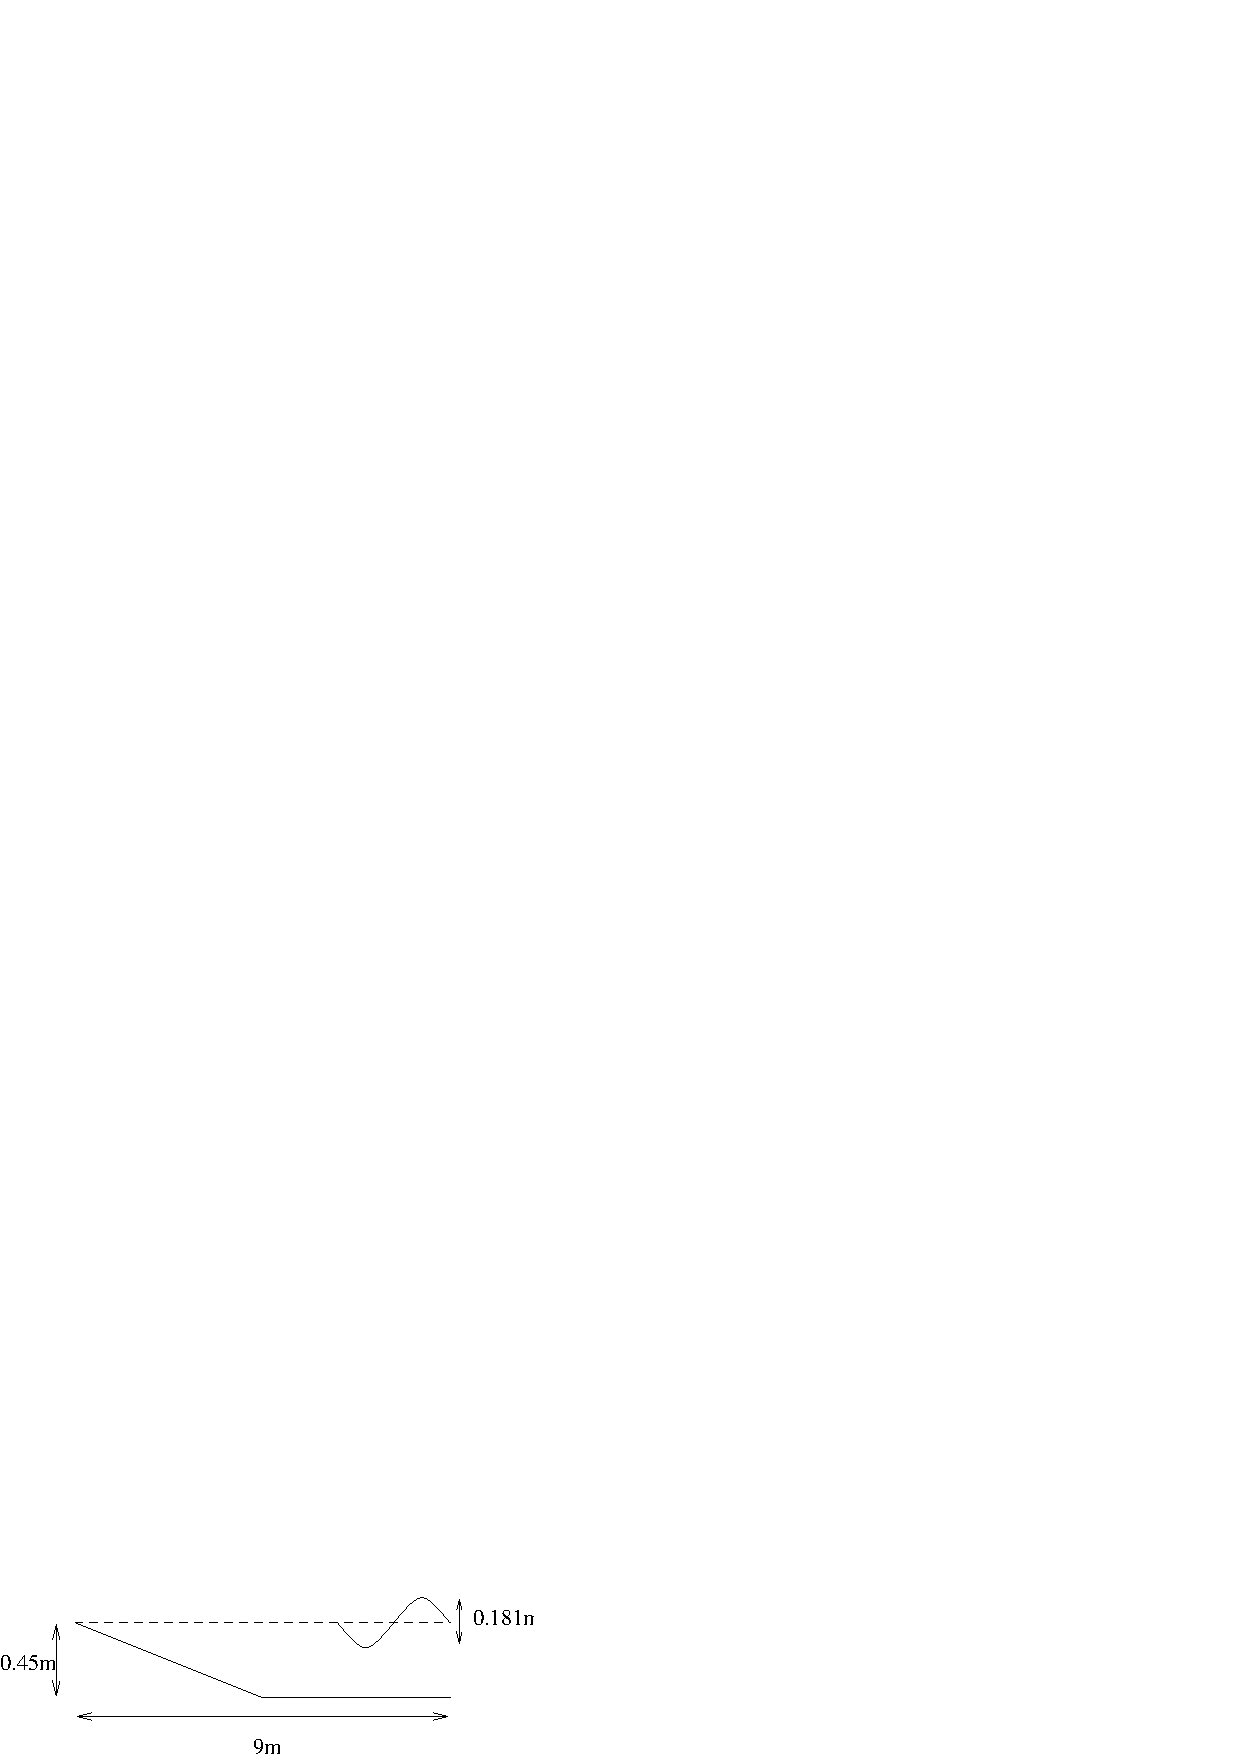
\includegraphics{FIG_wave/XIAsetup.pdf}}\par
\end{minipage}
\end{center}
\item The significant wave height satisfies to the two constraints:
\begin{equation*}
\begin{array}{rcl}
H_S^2 c_g  &=& Cst\mbox{~if~no~wave~energy~dissipation},\\
H_S & \leq & c_B (h +z) \mbox{~with~} c_B = 0.415.
\end{array}
\end{equation*}
\item The stress balance equation is
\begin{equation*}
\frac{\partial S_{xx}}{\partial x} = - \frac{1}{h+z} \frac{\partial h}{\partial x}
\end{equation*}
with $S_{xx}$ the Longuet-Higgins potential, $h$ the depth and $z$ the free surface.
\item The equation system can be solved very accurately.
\end{itemize}
}





\frame{
  \frametitle{Shoaling idealized test case II}

\begin{center}
\begin{minipage}{5.2cm}
\centering
\resizebox{5.0cm}{!}{\includegraphics[trim=15mm 5mm 15mm 10mm, clip]{FIG_wave/Zeta.png}}\par
Free surface
\end{minipage}
\begin{minipage}{5.2cm}
\centering
\resizebox{5.0cm}{!}{\includegraphics[trim=15mm 5mm 15mm 10mm, clip]{FIG_wave/Hsignificant.png}}\par
Significant wave height
\end{minipage}
%\begin{minipage}{10.2cm}
%\centering
%\resizebox{10.0cm}{!}{\includegraphics[trim=15mm 5mm 15mm 10mm, clip]{FIG_wave/Lwave.png}}\par
%Wave length
%\end{minipage}
\end{center}
}


\frame{
  \frametitle{Visser's idealized test case}
\begin{itemize}
\item Another important test case is Visser's test case where the waves are arriving obliquely on the beach. A longshore current is induced by the waves and it is balanced by dissipation in the model.
\item In order to adequately model such situations, we introduce ideal grid, that is grids where the model does not see the whole coordinate system:
\begin{itemize}
\item Input contains triangle area, list of nodes and node depth.
\item Differences of coordinates between nodes of each triangles.
\end{itemize}
%Everything (angle masks, differentials, ...) can be computed from this grid data.
%\item This allows to build periodic grids for coupled wave models and so to simulate academic test cases with the coupled system.
%\item When the model is in steady state a longshore current is induced by the waves and this current is balanced by dissipation in the model. See below results for Longuet-Higgins formulation:
\end{itemize}
\begin{center}
\begin{minipage}[t]{5.5cm}
\centering
\resizebox{4.5cm}{!}{\includegraphics[trim=15mm 10mm 15mm 10mm, clip]{FIG_wave/PictureVisser/Umagnitude.png}}\par
Longshore current
\end{minipage}
\end{center}

%\begin{center}
%\begin{minipage}[t]{10.5cm}
%\centering
%\resizebox{10.0cm}{!}{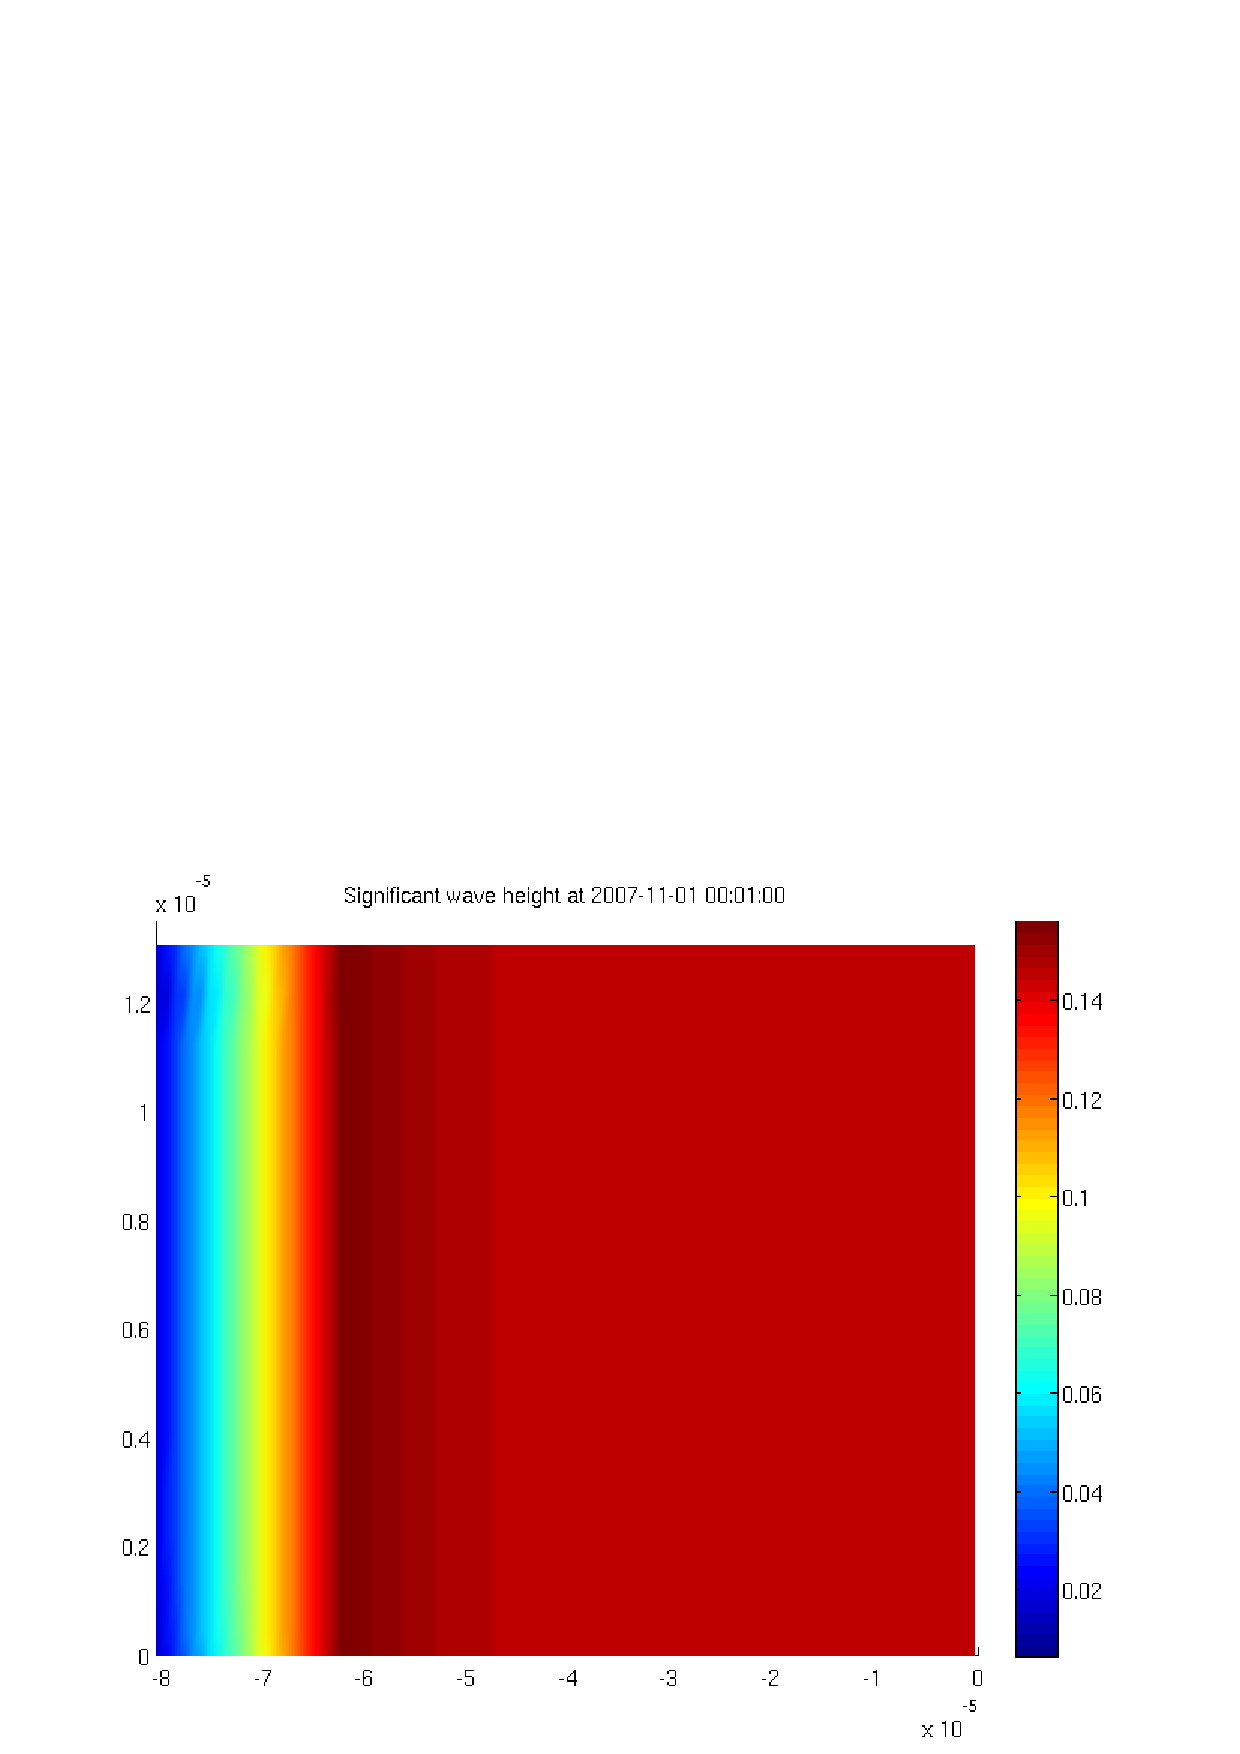
\includegraphics[trim=20mm 10mm 15mm 10mm, clip]{FIG_wave/PictureVisser/Hwave61_20071101_000100.png}}\par
%Significant wave height
%\end{minipage}
%\begin{minipage}[t]{10.5cm}
%\centering
%\resizebox{10.0cm}{!}{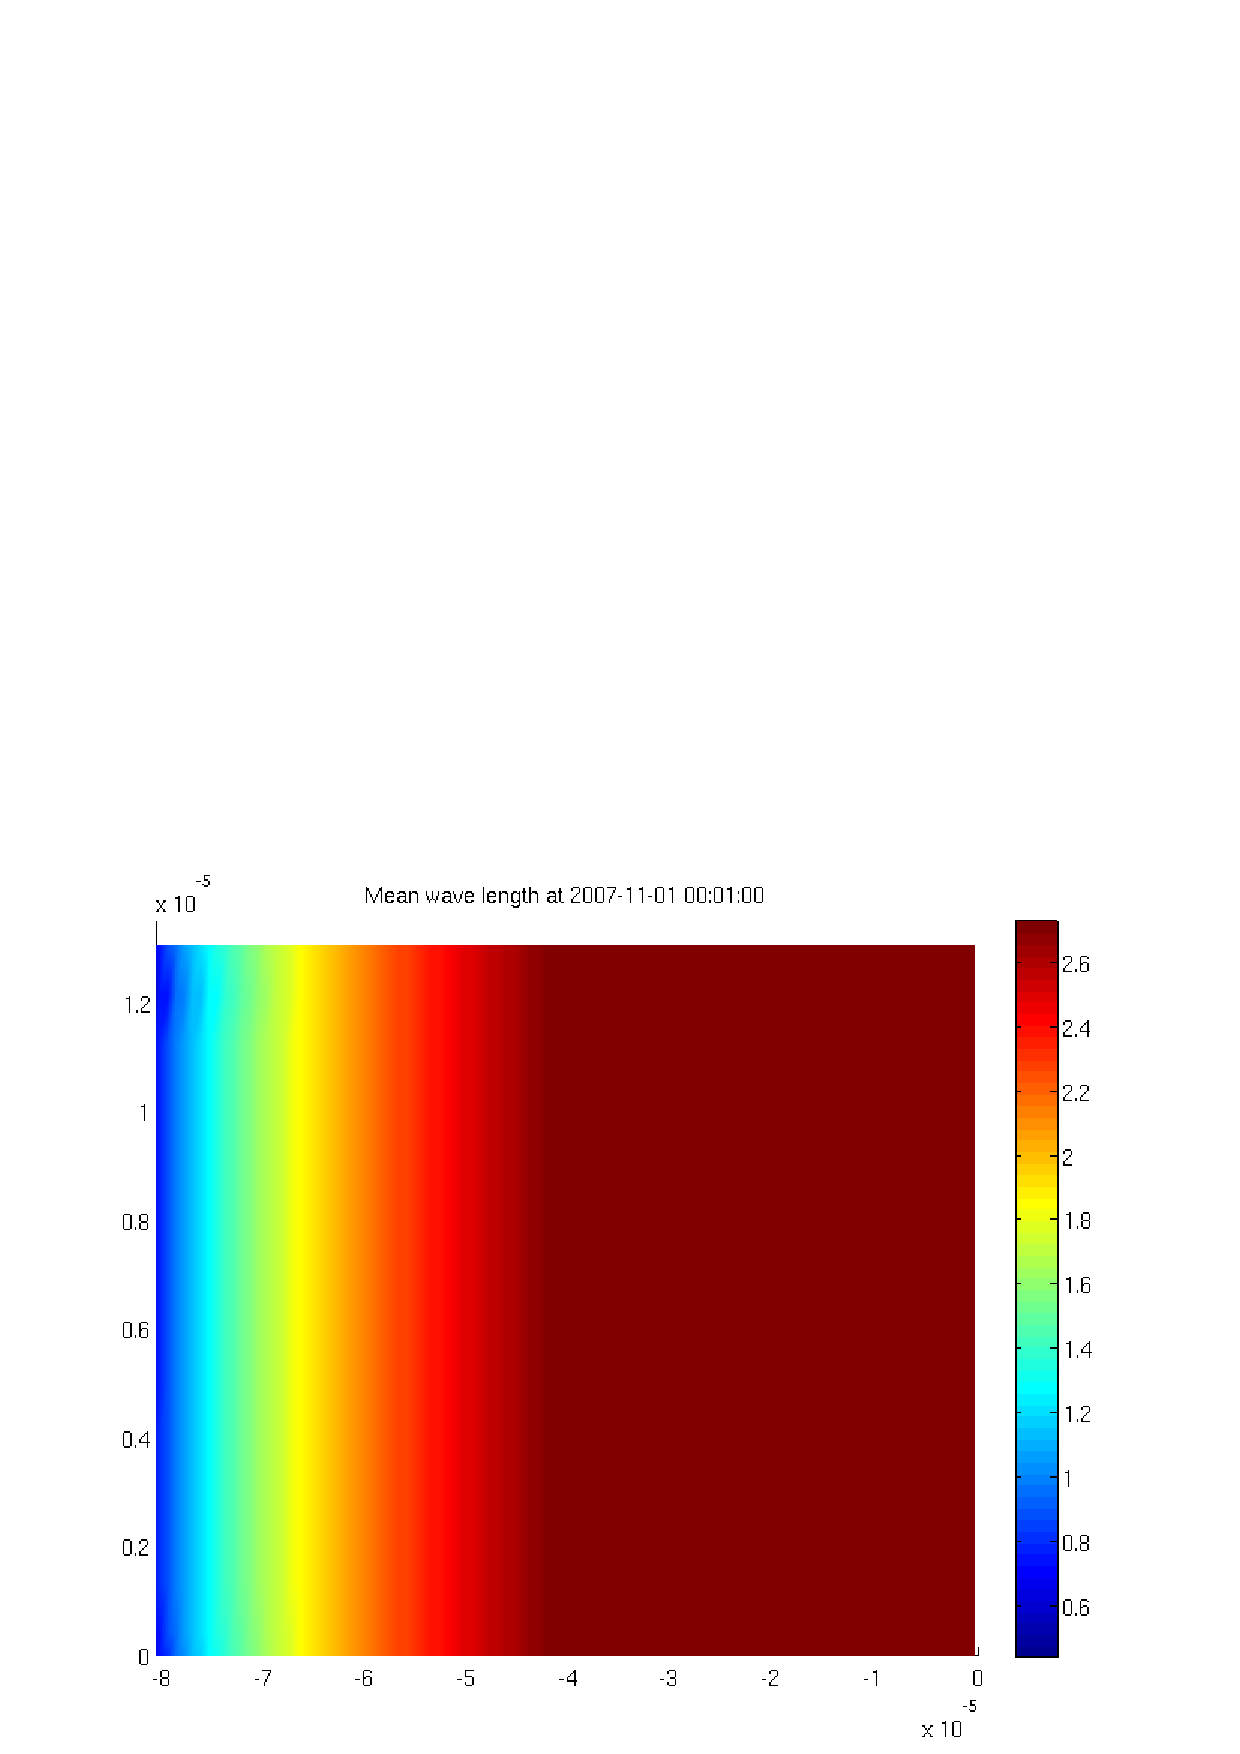
\includegraphics[trim=20mm 10mm 15mm 10mm, clip]{FIG_wave/PictureVisser/Lwave61_20071101_000100.png}}\par
%Wave length
%\end{minipage}
%\begin{minipage}[t]{10.5cm}
%\centering
%\resizebox{10.0cm}{!}{\includegraphics[trim=15mm 10mm 15mm 10mm, clip]{FIG_wave/PictureVisser/Umagnitude.png}}\par
%Longshore current
%\end{minipage}
%\begin{minipage}[t]{10.5cm}
%\centering
%\resizebox{10.0cm}{!}{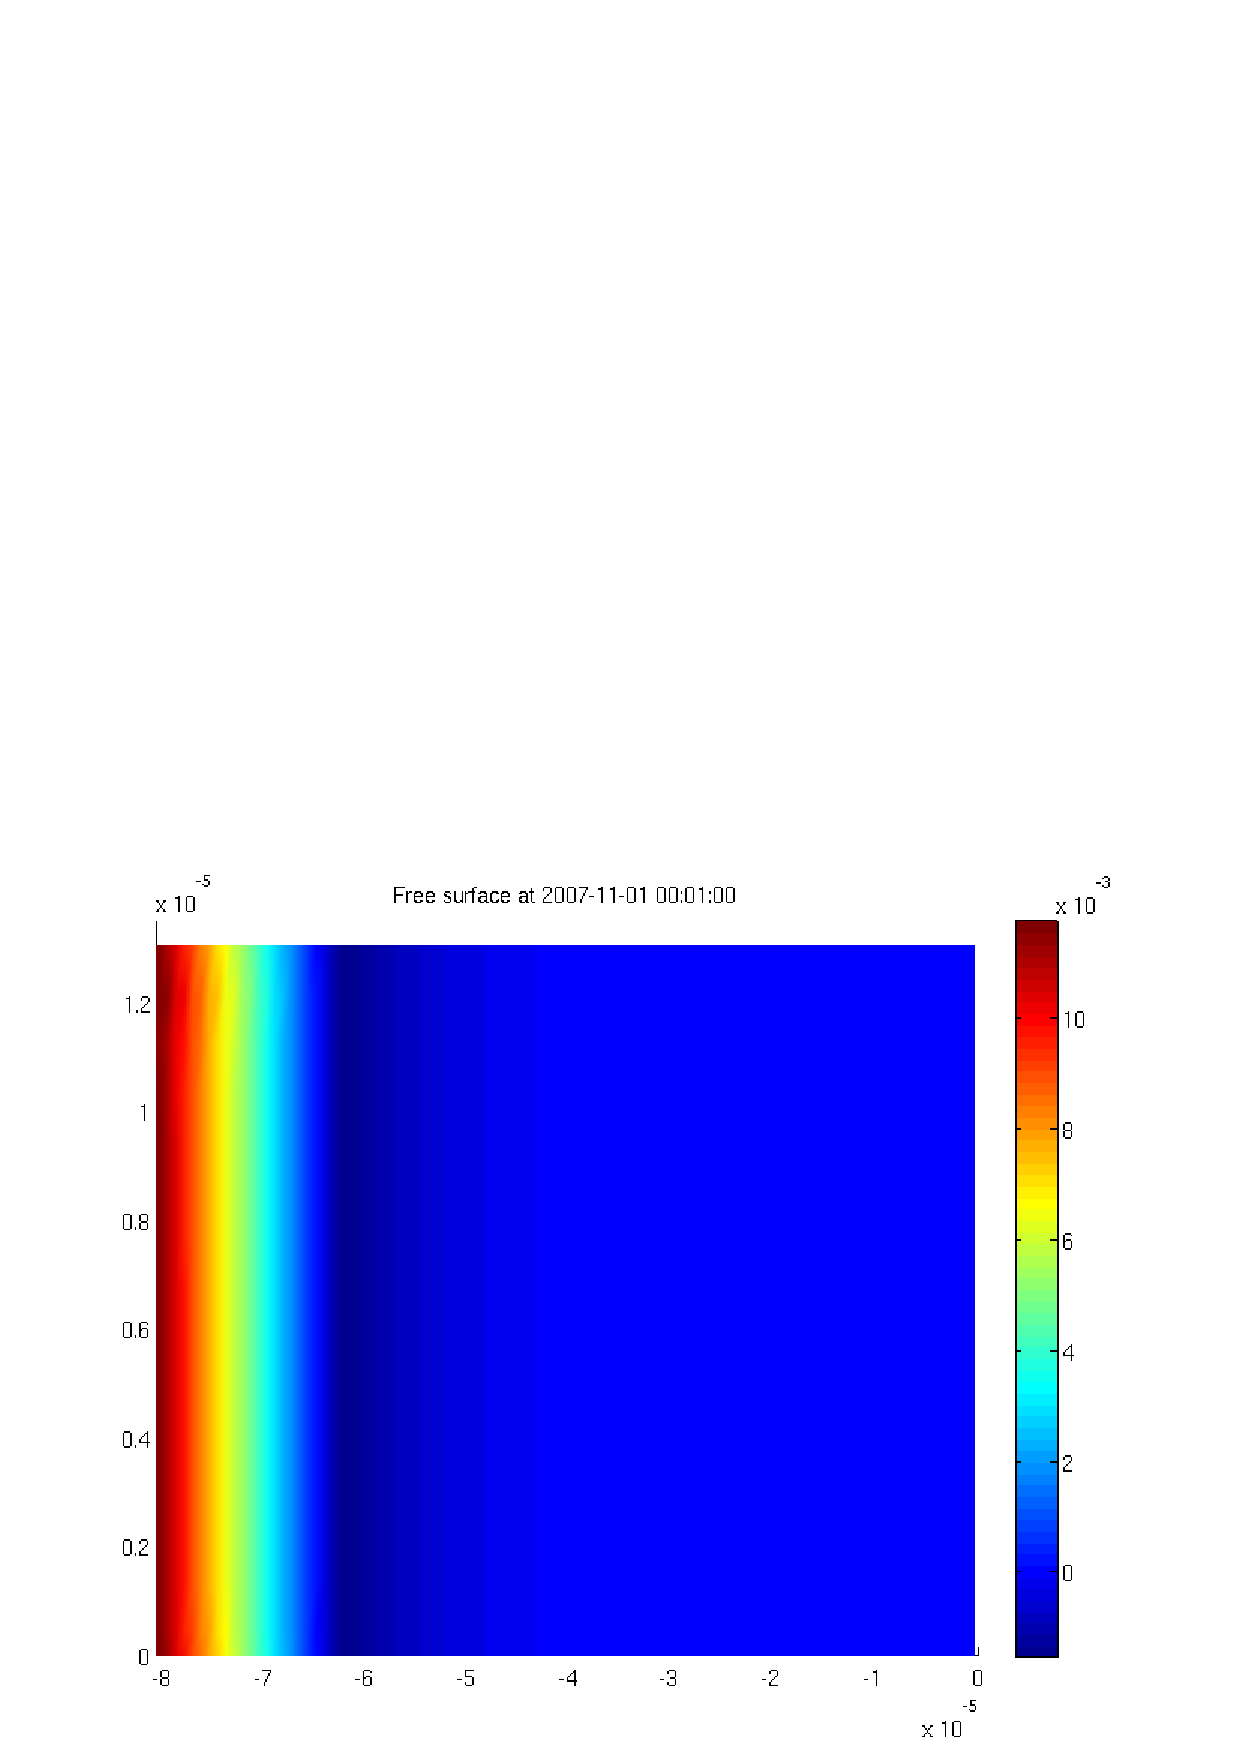
\includegraphics[trim=20mm 10mm 15mm 10mm, clip]{FIG_wave/PictureVisser/Zeta61_20071101_000100.png}}\par
%Free surface
%\end{minipage}
%\end{center}
}





\frame{
\begin{center}
\begin{tabular*}{10cm}{c}
\\[-0.5cm]
{\Huge \textcolor{blue}{IV. }\textcolor{red}{Hindcasting the state of}}\\[4mm]
{\Huge \textcolor{red}{the Adriatic Sea}}
\end{tabular*}
\end{center}
}


\frame{
  \frametitle{Bathymetry and rivers of the Adriatic Sea}

\begin{itemize}
\item The bathymetry varies a lot from 1200m to 50m.
\item The island structure on the Croatian side is quite complex.
\item River inflow is more important than in other parts of the Mediterranean.
\end{itemize}

\begin{center}
\begin{minipage}[b]{5.3cm}
%l b r t
\resizebox{5.2cm}{!}{\includegraphics[trim=35mm 11mm 35mm 11mm, clip]{PictureElect/BathymetryRiver.png}}\par
%\resizebox{5.5cm}{!}{\includegraphics[bb=101 32 477 403, clip]{PictureElect/BathymetryRiver.pdf_V1}}\par
\end{minipage}
\begin{minipage}[b]{5.3cm}
\begin{itemize}
\item Significant inflow/outflow occurs at the Ottranto strait and generates the highest tides of the Mediterranean.
\item Two winds Bora and Sirocco dominate the general circulation.
\end{itemize}
\end{minipage}
\end{center}

}




%\frame{
%  \frametitle{General circulation in the Adriatic Sea}
%
%\begin{itemize}
%\item The Mediterranean Sea exerts a significant influence at the Ottranto strait on the general circulation in the Adriatic.
%\item The tides are the highest in the Mediteranean sea.
%\end{itemize}
%}

%\frame{
%  \frametitle{A grid and the bathymetry}
%NEED TO CLEAN the HIGHER PART AND PUT gradation
%\vspace{-0.4cm}
%\begin{center}
%\resizebox{10.0cm}{!}{\includegraphics[bb=0 165 612 649, clip]{OceanPic/LogGridRich.pdf}}\par
%\epsfig{file=OceanPic/LogGridRich.pdf, height=13cm}
%\end{center}
%}



\frame{
  \frametitle{Chosen forcing information}

\begin{itemize}
\item The chosen modelization of the Adriatic Sea uses the atmospheric forcing fields from {\tt DHMZ} using the {\tt ALADIN} model (sea surface pressure, temperature, humidity, rain, cloud factor, short wave radiation).
\item For river forcing, we used:
\begin{itemize}
\item Hourly measurements for Po river and Neretva river.
\item Daily flux measurements for 9 other rivers and temperature for 5 more.
\item For other Italian rivers, we used climatological information from Raicich, 1994. For other Croatian rivers we rescale according to Neretva inflow.
\item For temperature we took nearest river.
\end{itemize}
\item We used an initial state obtained from {\tt AREG} which is an operational model using a modification of {\tt POM}.
\item At the open boundary of the Ottranto strait, we used daily average from the {\tt AREG} model and we add tidal signal to it.
\end{itemize}
}


\frame{
  \frametitle{The {\tt ROMS} model}
The {\tt ROMS} model (by Hernan Arango) is a finite difference model that solves the Eulerian primitive equation in curvilinear coordinates.
\begin{equation*}
\frac{\partial u}{\partial t} +u\frac{\partial u}{\partial x}
+v\frac{\partial u}{\partial y}+w\frac{\partial u}{\partial z}
= {\bf F}
\end{equation*}
The {\tt ROMS} model:
\begin{itemize}
\item uses the hydrostatic and Boussinesq approximations,
\item uses sigma-coordinates for the vertical discretization,
\item uses the split-explicit method in order to resolve
fast surface waves with a barotropic model,
\item has a variety of high order schemes for momentum advection,
tracer advection, horizontal pressure gradient, etc.,
\item has infrastructure for coupling with other models
({\tt SWAN}, {\tt WRF}, etc.),
\item has 4DVAR assimilation capabilities (not used here),
\item has biological and sediment sub models (not used here).
\end{itemize}
There are some other branches {\tt ROMS UCLA} and {\tt ROMS IRD}.
}





\frame{
  \frametitle{Available measurements}

\begin{itemize}
\item Satellite \textcolor{blue}{AVHRR} measurements sea surface temperature are available every few hours but are affected by clouds.
\item Daily \textcolor{blue}{Medspiration} synthetic data sets at 2km resolution of foundation temperature are created from various mea\-su\-re\-ments and model output. {\tt RMSE} is about $0.4 deg$.
\item {\em In situ} \textcolor{blue}{CTD} measurements available from cruises (Nov 2007, Mar, Jun, Jul 2008) with a priori insignificant error.
%\item Sea level gauges are available.
%\item ADCP (Acoustic Doppler Current Profiler) measures of currents.
%\item Output of meteorological models are available to get forcing data.
\end{itemize}

\begin{center}
\resizebox{4cm}{!}{\includegraphics[bb=203 45 628 476, clip]{PictureElect/Stations300_noline.pdf}}\par
\end{center}
}


\frame{
  \frametitle{Results (\textcolor{blue}{CTD})}

\begin{itemize}
\item One problem is that \textcolor{blue}{CTD} measurements are done near the coast, exactly where the model is expected to be bad.
\item For the \textcolor{blue}{CTD} we found following results:
\begin{center}
\begin{tabular}{|c|c|c|c|c|c|c|}
\hline
Mean cruise & \multicolumn{2}{|c|}{Temperature (deg)} &\multicolumn{2}{|c|}{Salinity (PSU)}\\
date        & {\tt RMSE}  & {\tt ME}     &  {\tt RMSE}  & {\tt ME}    \\\hline
01-11-2007  & 1.18  &  0.84  &  0.47  & -0.17 \\
20-03-2008  & 0.61  &  0.33  &  0.69  & -0.30 \\
01-06-2008  & 0.92  & -0.21  &  0.92  & -0.44 \\
01-07-2008  & 1.38  & -0.37  &  0.79  & -0.41 \\\hline
\end{tabular}
\end{center}
\item Large error for November 2007 is explained by the time of spin up of the model in august 2008.
\item Summer is generally more difficult to model appropriately due to stronger stratification.
\item Also problematic for modelling are narrow straits between islands.
\end{itemize}
}



\frame{
  \frametitle{Results (\textcolor{blue}{Medspiration})}


\begin{itemize}
\item No \textcolor{blue}{Medspiration} products were available for April and May.
\item Foundation temperature is compared with model temperature at 3 UTC.
\item For \textcolor{blue}{Medspiration} we found following results for {\tt RMSE}:
\begin{center}
{\scriptsize
\begin{tabular}{|c|c|c|c|c|}
\hline
Month     & North & Middle & South & Whole \\\hline
January   & 0.86  & 0.82   & 0.73  & 0.79\\
February  & 0.87  & 0.63   & 0.63  & 0.69\\
March     & 0.70  & 0.57   & 0.52  & 0.58\\
June      & 1.33  & 0.82   & 0.80  & 0.96\\
July      & 0.89  & 0.93   & 0.95  & 0.93\\
August    & 0.68  & 0.81   & 0.98  & 0.85\\
September & 1.09  & 1.00   & 1.02  & 1.03\\
October   & 0.57  & 0.79   & 0.70  & 0.71\\
Whole     & 0.90  & 0.79   & 0.80  & 0.82\\\hline
\end{tabular}
}
\end{center}
\item Mean error is generally very small except in June where it reaches $-0.40 deg$.
\item The \textcolor{blue}{Medspiration} product itself is not a measurement and when no {\tt AVHRR} scene is available, it then uses microwave sensors.
\end{itemize}
}





\frame{
  \frametitle{Comparison with QuikSCAT}

\begin{itemize}
\item QuikSCAT scatterometer provides sea surface neutral ($10m$) wind field at a $12.5km$ resolution.
\item When running the ROMS model, the stability contribution are computed and we thus get estimates of neutral winds.
\item Instrument specification gives zero bias and {\tt RMSE} $2m/s$ and $20deg$ for magnitude and direction.
Validation studies with {\em in situ} data in coastal region ($<80km$) show larger error ($0.93 \pm 1.83 m/s$) and ($4.71 \pm 31.15 deg$) (Tang et al., 2004).
\item Validation of ALADIN data with QuikSCAT data shows
\begin{center}
speed:   $-1.15 \pm 2.50 m/s$, 
direction:  $-4.16 \pm  38.14 deg$
\end{center}
\end{itemize}

\begin{center}
\begin{minipage}{10.2cm}
\centering
\resizebox{8.5cm}{!}{\includegraphics[trim=7mm 151mm 7mm 3mm, clip]{FIG_wave/ALD_QS_spatial_comparison.png}}\par
\end{minipage}
%\begin{minipage}{23.2cm}
%\centering
%\resizebox{23.0cm}{!}{\includegraphics[trim=25mm 25mm 32mm 145mm, clip]{FIG_wav%e/ALD_QS_spatial_comparison.png}}\par
%\end{minipage}
\end{center}
}


\frame{
  \frametitle{Comparison of Charnock coefficient}
\begin{center}
\epsfig{file=DrifterPicture/Scatter_Charnock/Scatter_bulk_wave.png, height=50mm}\par
\end{center}
\begin{itemize}
\item We see that the bulk formulation introduce an artificial looking Charnock coefficient with no spreading.
\item The wave formulation used here is the Ardhuin et al, (2009).
\end{itemize}
}




\frame{
  \frametitle{Comparison with wave stations I}

\begin{center}
Comparison with station $S$\par
{\scriptsize
\begin{tabular}{|c|ccc|ccc|cc|}
\hline
parameterization & \multicolumn{3}{|c|}{Significant wave height} & \multicolumn{3}{|c|}{Mean wave length} & \multicolumn{2}{|c|}{Mean direction}\\
\hline
          & {\tt RMSE} & {\tt ME} & Corr   & {\tt RMSE}  & {\tt ME} & Corr   & {\tt ME} & {\tt RMSE}\\
\hline
Cycle III & 0.26 & 0.09 & 0.87 & 24.55 & 20.55 & 0.68 & -1.77 & 60.51\\   
Cycle IV  & 0.27 & 0.10 & 0.86 & 19.43 & 15.83 & 0.72 & 4.29 & 56.45\\
Nedwam    & 0.23 & 0.01 & 0.88 & 20.17 & 14.54 & 0.73 & 7.83 & 55.74\\
Babanin   & 0.25 & 0.01 & 0.86 & 20.23 & 16.29 & 0.73 & 14.62 & 66.50\\
\hline
\end{tabular}
}
\end{center}
\vspace{0mm}
\begin{center}
Comparison with buoy $B$\par
{\scriptsize
\begin{tabular}{|c|ccc|ccc|cc|}
\hline
parameterization & \multicolumn{3}{|c|}{Significant wave height} & \multicolumn{3}{|c|}{Mean wave length} & \multicolumn{2}{|c|}{Peak direction}\\
\hline
          & {\tt RMSE} & {\tt ME} & Corr   & {\tt RMSE}  & {\tt ME}    & Corr   & {\tt ME} & {\tt RMSE}\\
\hline
Cycle III & 0.24 & 0.10 & 0.90 & 17.17 & 15.30 & 0.70 & -0.98 & 61.58\\
Cycle IV  & 0.23 & 0.09 & 0.90 & 10.60 & 8.73  & 0.79 & 3.94 & 64.09\\
Nedwam    & 0.20 &-0.01 & 0.92 & 11.42 & 9.48  & 0.76 & 2.16 & 63.48\\
Babanin   & 0.23 &-0.01 & 0.89 & 12.74 & 11.00 & 0.77 & 5.71 & 60.09\\
\hline
\end{tabular}
}
\end{center}
\begin{center}
Still more advanced physics is by Ardhuin etal. (2009).
\end{center}
}

\frame{
  \frametitle{Comparison with wave stations II}

\begin{center}
\begin{minipage}{5.2cm}
\centering
\resizebox{5.0cm}{!}{\includegraphics[trim=15mm 8mm 7mm 10mm, clip]{FIG_wave/Comp15ndImpl_4run_ISMAR_S1/BuoyFiles/ISMARtowerHwave/CombinedPicture_Hwave.png}}\par
\end{minipage}
\begin{minipage}{5.2cm}
\centering
\resizebox{5.0cm}{!}{\includegraphics[trim=15mm 8mm 7mm 10mm, clip]{FIG_wave/Comp15ndImpl_4run_ISMAR_S1/BuoyFiles/ISMARtowerLwave/CombinedPicture_Lwave.png}}\par
\end{minipage}
\end{center}
\begin{center}
\begin{minipage}{5.2cm}
\centering
\resizebox{5.0cm}{!}{\includegraphics[trim=15mm 8mm 7mm 10mm, clip]{FIG_wave/Comp15ndImpl_4run_ISMAR_S1/BuoyFiles/V1_11_2007_08_2008smoHwave/CombinedPicture_Hwave.png}}\par
Significant wave height
\end{minipage}
\begin{minipage}{5.2cm}
\centering
\resizebox{5.0cm}{!}{\includegraphics[trim=15mm 8mm 7mm 10mm, clip]{FIG_wave/Comp15ndImpl_4run_ISMAR_S1/BuoyFiles/V1_11_2007_08_2008smoLwave/CombinedPicture_Lwave.png}}\par
Mean wave length
\end{minipage}
\end{center}
}

\frame{
  \frametitle{Grids of the Adriatic}
%trim=l b r t
\begin{center}
\begin{minipage}{5.2cm}
\resizebox{5.2cm}{!}{\includegraphics[bb=166 390 399 555,clip]{FIG_wave/Stations300_AASSb.pdf}}\par
\end{minipage}
\begin{minipage}{5.2cm}
\resizebox{6.3cm}{!}{\includegraphics[trim=16mm 28mm 16mm 28mm, clip]{FIG_wave/PicCompar/RomsGrid.png}}\par
\end{minipage}
\end{center}
\begin{center}
\begin{minipage}{5.2cm}
\resizebox{5.8cm}{!}{\includegraphics[trim=16mm 28mm 16mm 28mm, clip]{FIG_wave/PicCompar/FEMgrid1.png}}\par
\end{minipage}
\begin{minipage}{5.2cm}
\resizebox{5.8cm}{!}{\includegraphics[trim=16mm 28mm 16mm 28mm, clip]{FIG_wave/PicCompar/FEMgrid2.png}}\par
\end{minipage}
\end{center}
}





\frame{
  \frametitle{Mean absolute error between grid {\tt UG1} and {\tt UG2} I}

\begin{center}
\begin{minipage}{5.3cm}
\centering
\resizebox{5.5cm}{!}{\includegraphics[trim=23mm 10mm 23mm 10mm, clip]{FIG_wave/DiffPictures/HwaveDiff.png}}\par
Significant wave height
\end{minipage}
\begin{minipage}{5.3cm}
\centering
\resizebox{5.5cm}{!}{\includegraphics[trim=23mm 10mm 23mm 10mm, clip]{FIG_wave/DiffPictures/LwaveDiff.png}}\par
Mean wave length
\end{minipage}
\end{center}
\begin{itemize}
\item The grid impact on Significant wave height is very small.
\item It is larger for Mean wave length, but still reasonable.
\end{itemize}
}

\frame{
  \frametitle{Mean absolute error between grid {\tt UG1} and {\tt UG2} II}
\begin{center}
\begin{minipage}{5.3cm}
\centering
\resizebox{5.5cm}{!}{\includegraphics[trim=23mm 10mm 23mm 10mm, clip]{FIG_wave/DiffPictures/DwaveDiff.png}}\par
Mean wave direction
\end{minipage}
\begin{minipage}{5.3cm}
\centering
\resizebox{5.5cm}{!}{\includegraphics[trim=23mm 10mm 23mm 10mm, clip]{FIG_wave/DiffPictures/UVnormDiff.png}}\par
Surface current
\end{minipage}
\end{center}
\begin{itemize}
\item Wind direction is more unstable when the waves are smaller.
\item For surface current, we see that the Stokes drift is fairly important for the Western Adriatic Current.
%\item The future appears to be to go to unstructured models (Work in preparation with Y. Zhang and A. Roland on coupling of {\tt SELFE} and {\tt WWM}).
\end{itemize}
Work done with A. Roland (TU Darmstadt), I. Toma\u zi\'c, I. Janekovi\'c, M. Kuzmi\'c (IRB).
}

\frame{
  \frametitle{Impact of various parameterizations}


\begin{center}
\begin{minipage}{5.3cm}
\centering
\resizebox{5.5cm}{!}{\includegraphics[trim=23mm 10mm 23mm 10mm, clip]{WavePic/Comp_ADCP_ivD_detide_N_Jan7_13b/KB1/KB1_uv_surf_mag_detide_CombiPic_uv_surf_mag_detide.png}}\par
\end{minipage}
\begin{minipage}{5.3cm}
\centering
\resizebox{5.5cm}{!}{\includegraphics[trim=23mm 10mm 23mm 10mm, clip]{WavePic/Comp_ADCP_ivD_detide_N_Jan7_13b/VR2/VR2_uv_surf_mag_detide_CombiPic_uv_surf_mag_detide.png}}\par
\end{minipage}
\end{center}
Surface current magnitude with increasing coupling at $KB1$ and $VR2$
}





\frame{
%  \frametitle{Thank you}
\vspace{1.5cm}
\begin{center}
{\Huge \textcolor{red}{T}\textcolor{blue}{H}\textcolor{green}{A}\textcolor{blue}{N}\textcolor{red}{K}}\\[1cm]
{\Huge \textcolor{red}{Y}\textcolor{blue}{O}\textcolor{red}{U}}
%\epsfig{file=plit-gal10.eps, height=5.5cm}
\end{center}
}




\end{document}
